%==================================================================
% Ini adalah bab 3
% Silahkan edit sesuai kebutuhan, baik menambah atau mengurangi \section, \subsection
%==================================================================

\chapter[KONSEP RANCANGAN / PRODUK / JASA / EVALUASI / PENGUJIAN]{\\ KONSEP RANCANGAN / PRODUK / JASA / EVALUASI / PENGUJIAN}

\section{Section 3.1}
Desain penelitian adalah bagian penting dari laporan proyek akhir sarjana terapan yang menjabarkan tentang rencana dan perencanaan yang digunakan dalam melakukan penelitian. Desain penelitian harus jelas dan terukur, sehingga dapat membantu dalam menjawab masalah yang diteliti. Desain penelitian terdiri dari beberapa elemen, seperti desain penelitian, metode pengumpulan data, sampel, dan analisis data.

Desain penelitian dalam laporan proyek akhir sarjana terapan harus mempertimbangkan beberapa hal, seperti:
\begin{packed_item}
    \item Masalah yang diteliti
    \item Tujuan penelitian
    \item Populasi dan sampel yang digunakan
    \item Metode pengumpulan data
    \item Analisis data yang digunakan
\end{packed_item}

Dalam laporan proyek akhir sarjana terapan yang meneliti pengaruh perubahan iklim terhadap hasil panen padi, desain penelitian yang digunakan adalah desain eksperimen. Desain eksperimen digunakan karena dapat menguji hipotesis dengan mengontrol variabel bebas dan mengukur variabel terikat.

Desain eksperimen ini meliputi pemilihan lokasi penelitian yang sesuai dengan kondisi iklim yang berbeda, pembuatan plot percobaan, dan aplikasi pengaturan iklim yang berbeda pada plot percobaan. Metode pengumpulan data yang dapat digunakan adalah observasi, wawancara dan pengukuran parameter-parameter penting seperti suhu, curah hujan, dan kadar CO2. Sampel yang digunakan adalah tanaman padi yang ditanam di lokasi yang berbeda dengan kondisi iklim yang berbeda. Analisis data yang digunakan adalah statistik deskriptif dan inferensial untuk mengetahui pengaruh perubahan iklim terhadap hasil panen padi.

Implementasi adalah bagian dari laporan proyek akhir sarjana terapan yang menjabarkan tentang pelaksanaan penelitian sesuai dengan rencana yang telah ditetapkan dalam desain penelitian. Implementasi meliputi tahap-tahap dari pelaksanaan penelitian, seperti pengambilan sampel, pengumpulan data, dan analisis data.

Implementasi dari desain penelitian tersebut dilakukan dengan cara mengambil sampel tanaman padi di lokasi yang berbeda dengan kondisi iklim yang berbeda, kemudian melakukan pengukuran parameter-parameter penting seperti suhu, curah hujan, dan kadar CO2. Kemudian data yang didapat dianalisis untuk mengetahui pengaruh perubahan iklim terhadap hasil panen padi.

Dalam proses implementasi, langkah-langkah yang dilakukan meliputi:

\begin{packed_enum}
    \item Pemilihan lokasi penelitian yang sesuai dengan kondisi iklim yang berbeda.
    \item Pembuatan plot percobaan dan pengaturan iklim yang berbeda pada plot percobaan.
    \item Pengambilan sampel tanaman padi di lokasi yang berbeda dengan kondisi iklim yang berbeda.
    \item Pengukuran parameter-parameter penting seperti suhu, curah hujan, dan kadar CO2.
    \item Analisis data yang didapat untuk mengetahui pengaruh perubahan iklim terhadap hasil panen padi.
    \item Implementasi harus dilakukan dengan benar dan teliti agar hasil yang didapat dapat diterima dan dipercaya. Selain itu, implementasi juga harus dilakukan secara objektif agar hasil yang didapat dapat diinterpretasikan dengan benar dan dapat digunakan untuk menjawab masalah yang diteliti.
\end{packed_enum}

Secara keseluruhan, desain dan implementasi adalah bagian penting dari laporan proyek akhir sarjana terapan yang membantu dalam menjabarkan rencana dan pelaksanaan penelitian yang dilakukan. Desain penelitian harus jelas dan terukur serta mempertimbangkan masalah yang diteliti, tujuan penelitian, sampel yang digunakan, metode pengumpulan data, dan analisis data yang digunakan. Implementasi harus dilakukan dengan benar dan teliti serta objektif agar hasil yang didapat dapat diterima dan dipercaya serta dapat digunakan untuk menjawab masalah yang diteliti.

\subsection{Subsection 3.1.1}
Bagian ini digunakan apabila dibutuhkan, silahkan bisa ditambah atau dikurangi sesuai kebutuhan.

\subsection{Subsection 3.1.2}
Bagian ini digunakan apabila dibutuhkan, silahkan bisa ditambah atau dikurangi sesuai kebutuhan.

\subsection{Subsection 3.1.3}
Bagian ini digunakan apabila dibutuhkan, silahkan bisa ditambah atau dikurangi sesuai kebutuhan.

\section{Mengedit dokumen \LaTeX}
Pada bagian ini akan menjelaskan beberapa hal yang diperlukan ketika bekerja pada file \LaTeX.

\subsection{Menambahkan Gambar}
Untuk menambahkan gambar hal yang harus dilakukan adalah:
\begin{packed_enum}
    \item Menyalin file gambar (dalam format jpg \/ png) ke dalam folder \textit{gambar}
    \item Mengganti nama file dari gambar agar mudah dikenali, jangan diberi nama gambar-1,-2, dst
    \item Memasukkan kode di bawah
\end{packed_enum}

%\begin{lstlisting}[language=TeX]
%    \begin{figure}[H]
%        \centering
%        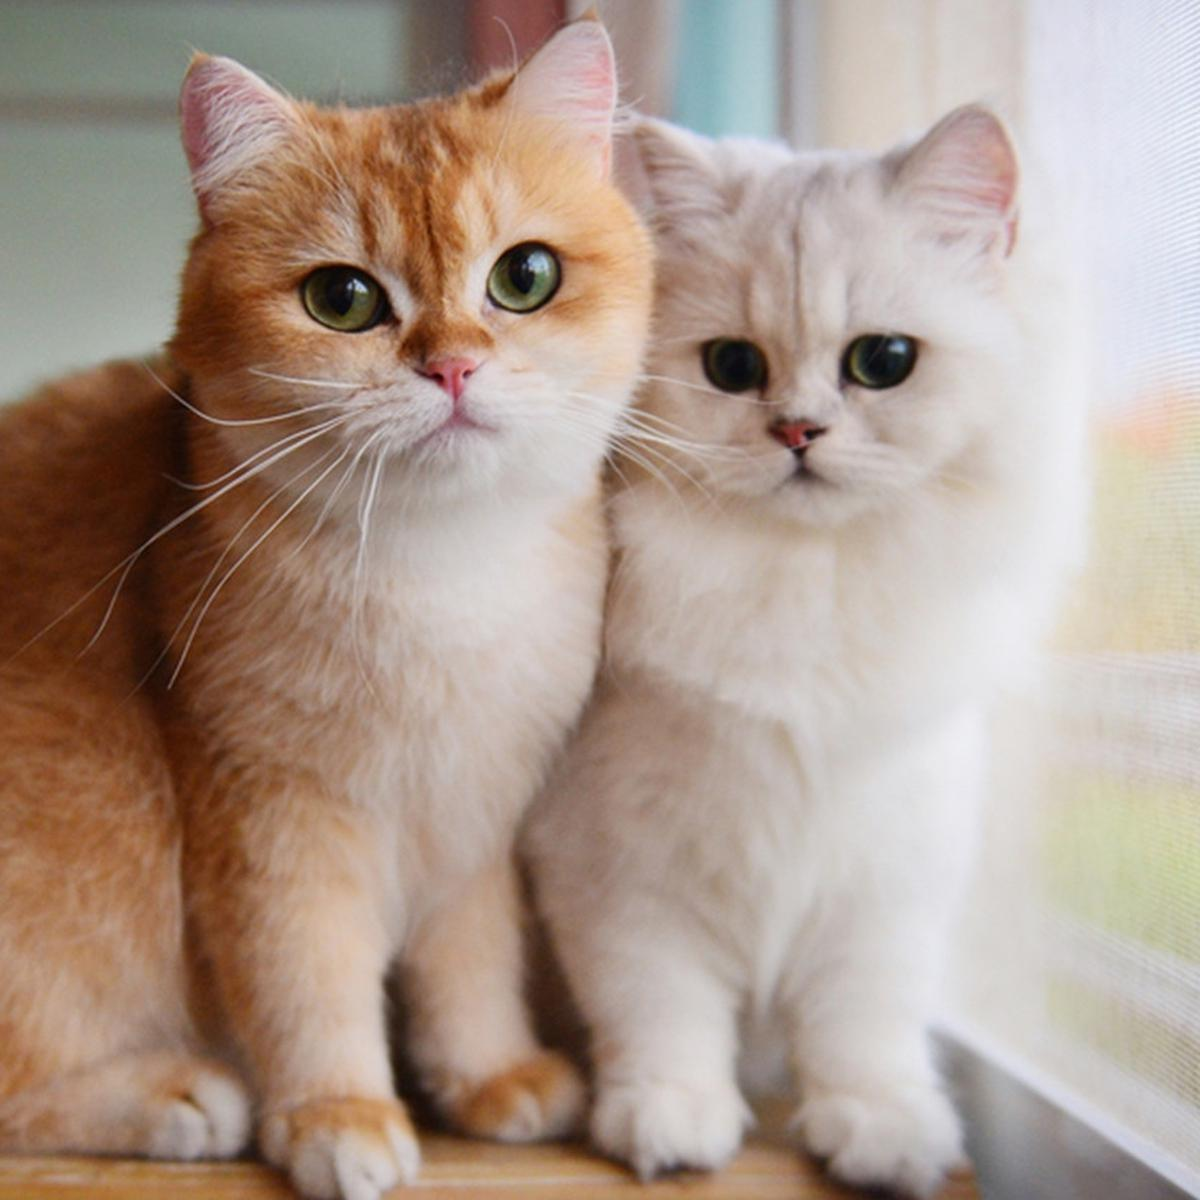
\includegraphics[scale=0.2]{gambar-kucing}
%        \caption{Gambar Kucing Lucu dan Imut}
%    \end{figure}
%\end{lstlisting}

Ukuran gambar dapat diganti dengan mengganti nilai pada scale. Jangan lupa memberikan caption pada setiap gambar. Berikut adalah contoh dari gambar yang telah dimasukkan pada dokumen. Penomoran gambar sudah otomatis dan akan masuk ke daftar gambar juga secara otomatis. Apabila ada beberapa gambar yang akan di embed dengan 1 caption, maka silahkan edit terlebih dahulu dan dijadikan menjadi 1 gambar. Posisi gambar akan pasti setelah dari text ini, apabila ingin mengganti posisinya parameter \textit{H} dapat diganti dengan \textit{h, t, b, p} sesuai kebutuhan.

\begin{figure}[H]
    \centering
    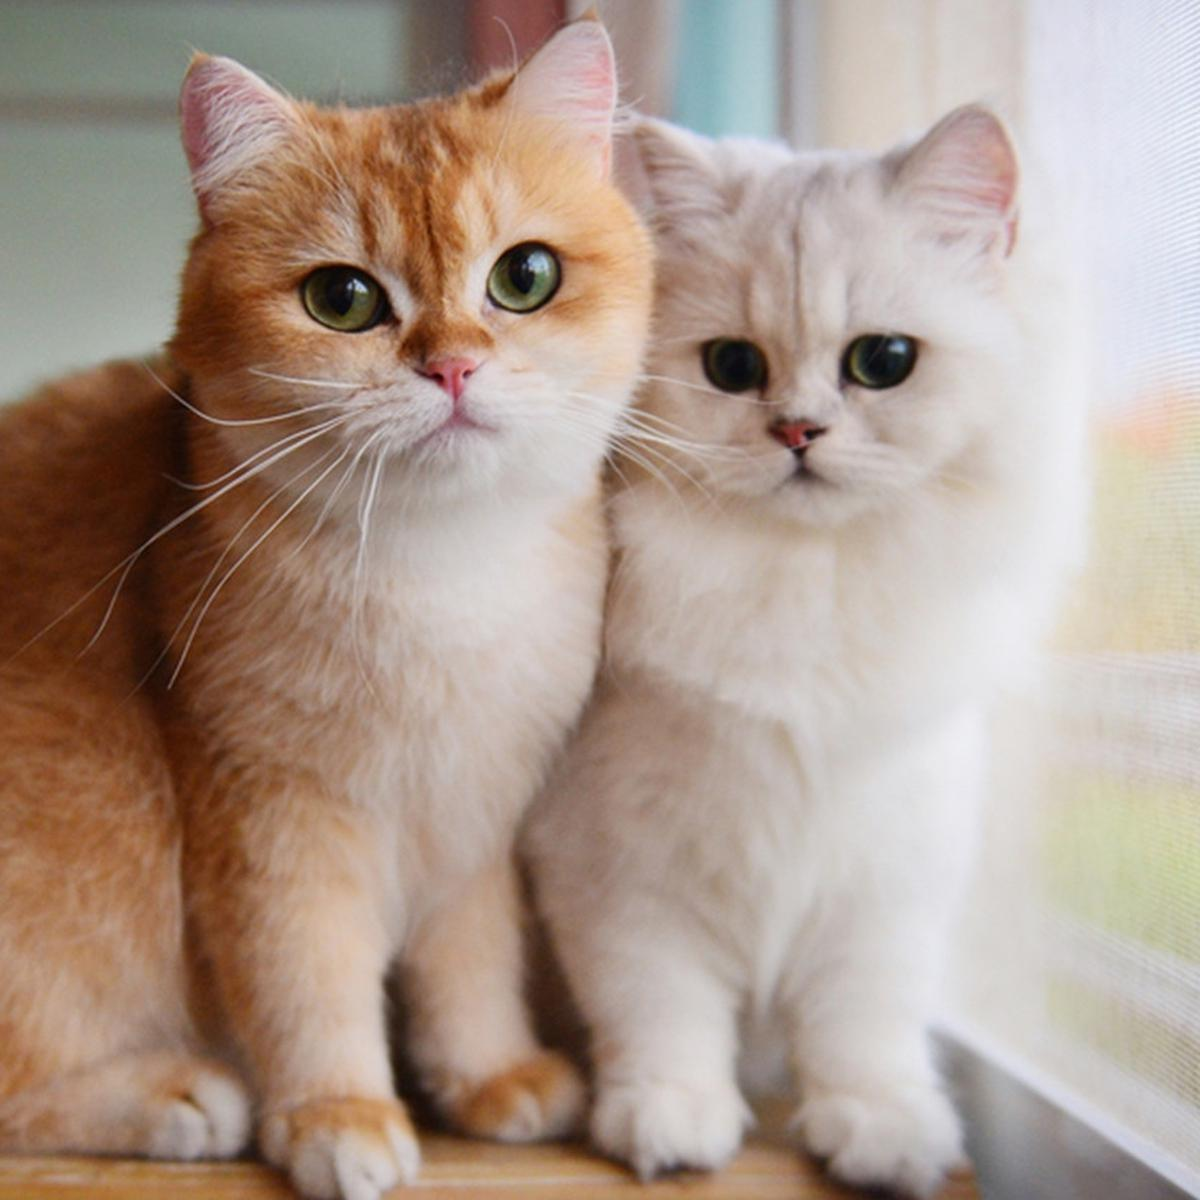
\includegraphics[scale=0.1]{gambar-kucing}
    \caption{Gambar Kucing Lucu dan Imut dengan scala 0.1}
    \label{fig:kucing}
\end{figure}

Setiap gambar harus dimention atau disebutkan didalam bacaan seperti berikut ini \cref{fig:kucing}.

\begin{figure}[H]
    \centering
    
\includegraphics[scale=0.4]{logo-uny}
    \caption{Logo UNY dengan scala 0.4}
    \label{fig:logoUNY}
\end{figure}

Untuk menambahkan gambar secara landscape dapat dilihat pada contoh berikut ini dan jangan lupa selalu menyebutkan nomor gambar disertai penjelasannya seperti ini \cref{fig:logoUNY} dan ini \cref{fig:kucingdanUNY}.

\begin{figure}
	\centering
	\begin{subfigure}[b]{0.3\textwidth}
		\centering
		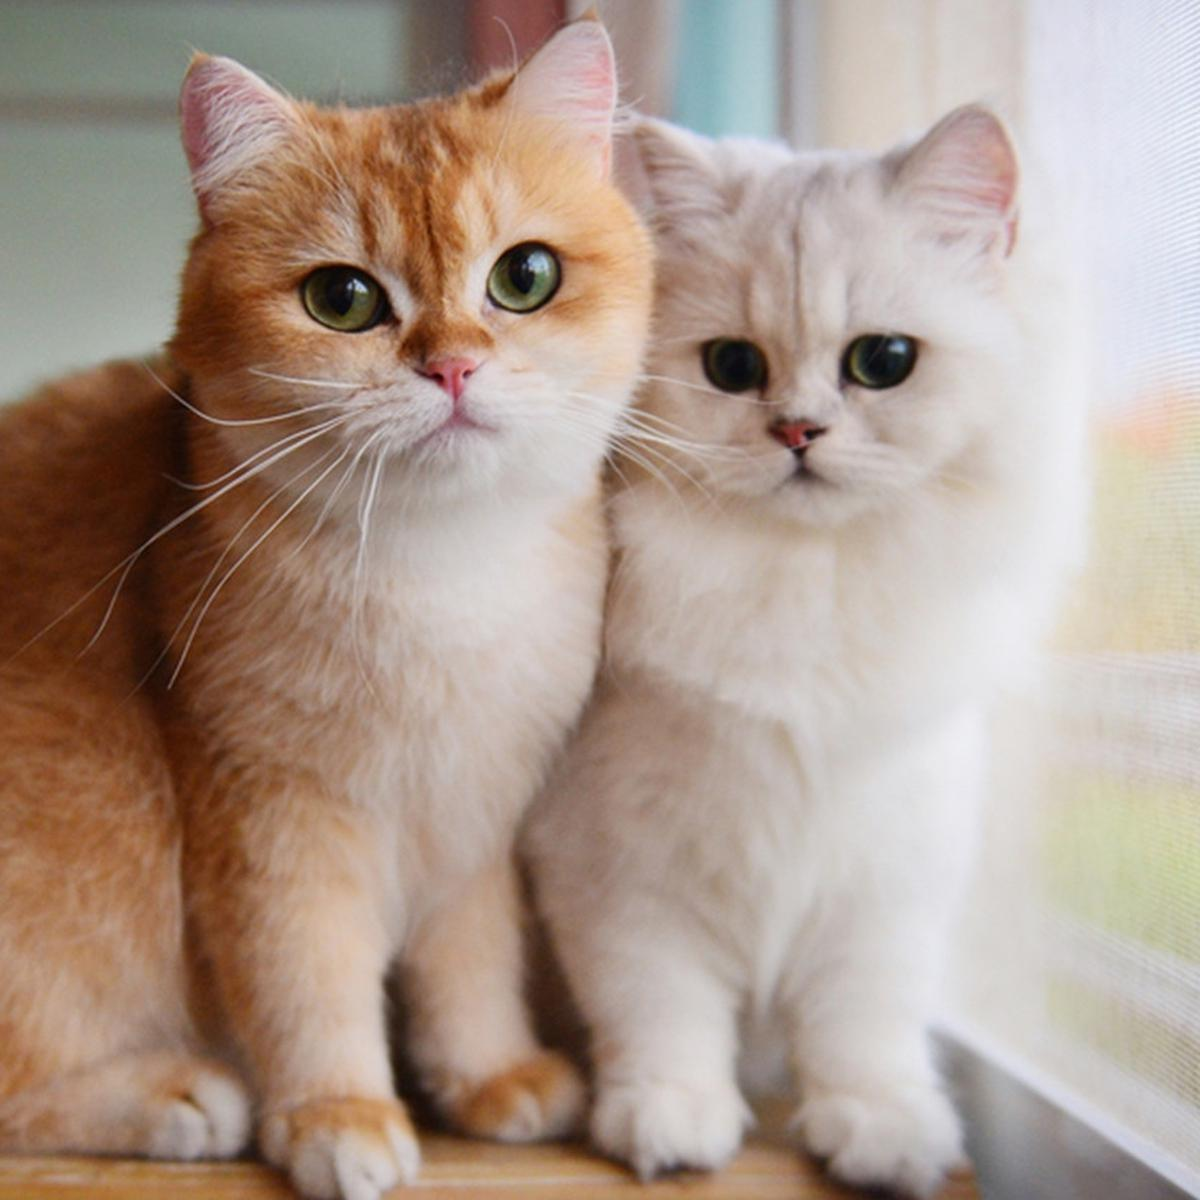
\includegraphics[width=\linewidth]{gambar-kucing}
		\caption{Kucing Lucu 1}
		\label{fig:kucing-a}
	\end{subfigure}
	\hfill
	\begin{subfigure}[b]{0.3\textwidth}
		\centering
		
\includegraphics[width=\linewidth]{logo-uny}
		\caption{Logo UNY}
		\label{fig:logo-uny-b}
	\end{subfigure}
	\hfill
	\begin{subfigure}[b]{0.3\textwidth}
		\centering
		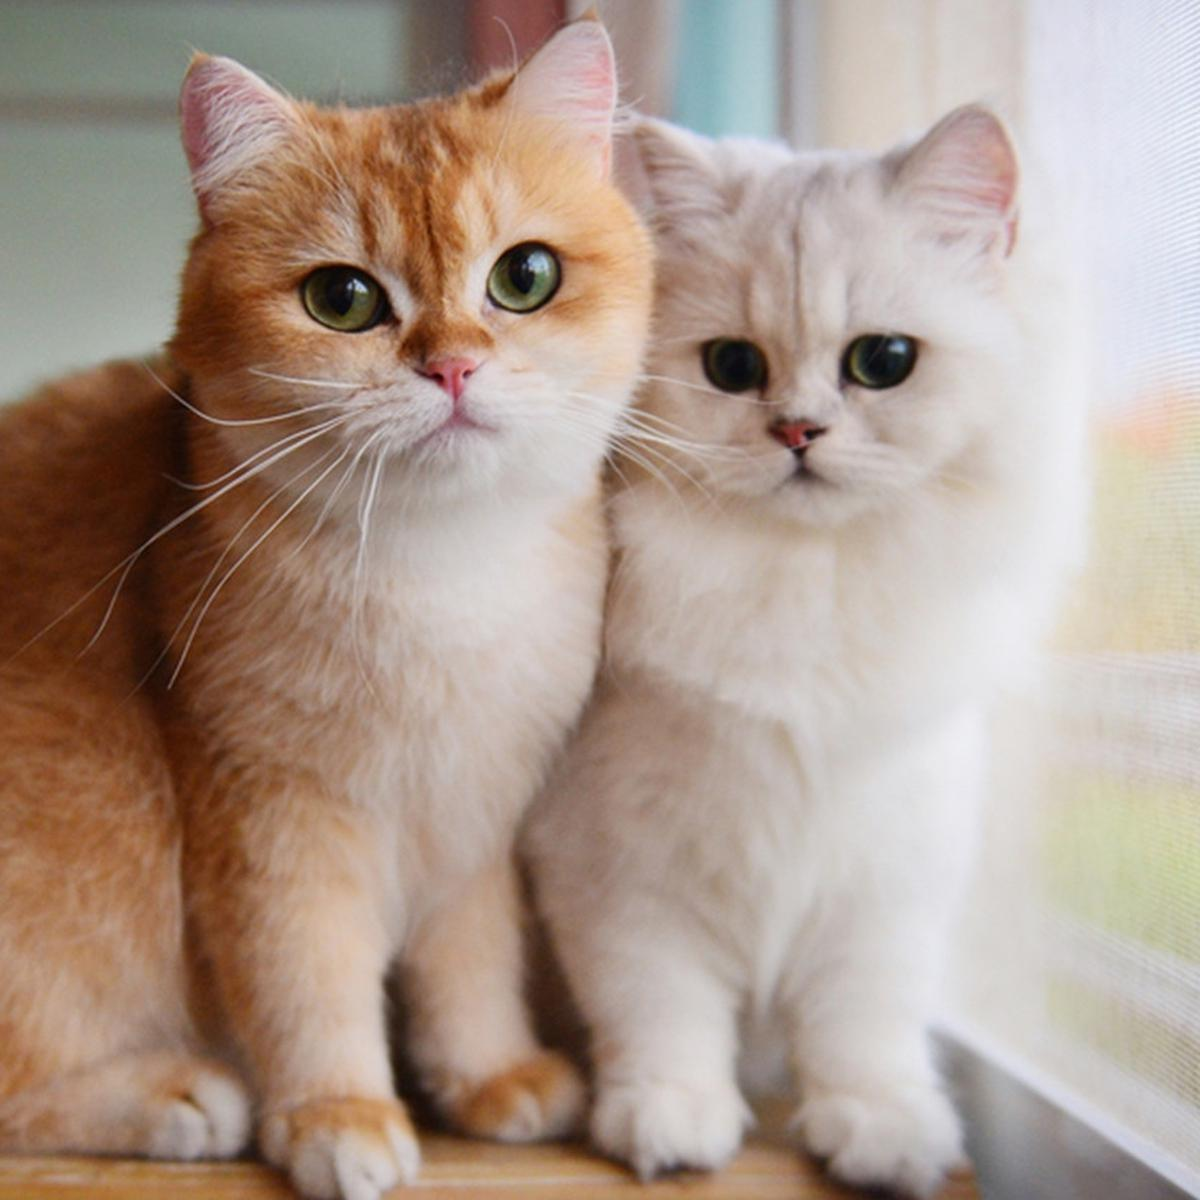
\includegraphics[width=\linewidth]{gambar-kucing}
		\caption{Kucing Lucu 2}
		\label{fig:kucing-c}
	\end{subfigure}
	   \caption{3 gambar yang disusun menjadi 1 bagian dengan penomoran (a), (b), dan (c)}
	   \label{fig:kucingdanUNY}
\end{figure}

\subsection{Membuat Tabel}
Pada bagian ini akan dijelaskan bagaimana membuat tabel dalam sebuah dokumen \LaTeX. untuk membuat tabel memang agak sedikit sulit, sehingga saya menyarankan menggunakan tool berikut \url{https://www.tablesgenerator.com/} atau \url{https://www.latex-tables.com/} kemudian isikan tabel pada tool generator tersebut dan salin kodenya ke dalam dokumen \LaTeX. Berikut adalah contoh dari sebuah tabel yang telah dibuat. Jangan lupa setiap tabel harus dimention dan dijelaskan dibacaan seperti berikut ini \cref{tab:hresult}.

\begin{table}[h]
	\caption{Performance Using Hard Decision Detection}
	\label{tab:hresult}
	\centering
	\begin{tabular}{c rrrrrrr}
		\hline\hline
		Audio Name&\multicolumn{7}{c}{Sum of Extracted Bits} \\ [0.5ex] 
		\hline
		Police & 5 & -1 & 5& 5& -7& -5& 3\\
		Midnight & 7 & -3 & 5& 3& -1& -3& 5\\
		News & 9 & -3 & 7& 9& -5& -1& 9\\[0.8ex]
		\hline
	\end{tabular}
\end{table}

Kita juga bisa menambahkan tabel yang besar dengan format halaman landscape seperti contoh berikut dan mention tabel seperti berikut ini \cref{tab:LPer} dan berikut ini \cref{tab:PPer}.

\begin{sidewaystable}[htbp]
	\caption{Performance After Post Filtering}
	\label{tab:LPer}
	\centering
	\begin{tabular}{l c c rrrrrrr}
		\hline\hline
		Audio &Audibility & Decision &\multicolumn{7}{c}{Sum of Extracted Bits} 
		\\ [0.5ex] 
		\hline
		& &soft &1 & $-1$ & 1 & 1 & $-1$ & $-1$ & 1 \\[-1ex]
		\raisebox{1.5ex}{Police} & \raisebox{1.5ex}{5}&hard
		& 2 & $-4$ & 4 & 4 & $-2$ & $-4$ & 4 \\[1ex]
		& &soft & 1 & $-1$ & 1 & 1 & $-1$ & $-1$ & 1 \\[-1ex]
		\raisebox{1.5ex}{Beethoven} & \raisebox{1.5ex}{5}& hard
		&8 & $-8$ & 2 & 8 & $-8$ & $-8$ & 6 \\[1ex]
		& &soft & 1 & $-1$ & 1 & 1 & $-1$ & $-1$ & 1 \\[-1ex]
		\raisebox{1.5ex}{Metallica} & \raisebox{1.5ex}{5}& hard
		&4 & $-8$ & 8 & 4 & $-8$ & $-8$ & 8 \\[1ex]
		\hline
	\end{tabular}
\end{sidewaystable}
	
\begin{table}[h]
	\caption{Performance After Post Filtering}
	\label{tab:PPer}
	\centering
	\begin{tabular}{l c c rrrrrrr}
		\hline\hline
		Audio &Audibility & Decision &\multicolumn{7}{c}{Sum of Extracted Bits} 
		\\ [0.5ex] 
		\hline
		& &soft &1 & $-1$ & 1 & 1 & $-1$ & $-1$ & 1 \\[-1ex]
		\raisebox{1.5ex}{Police} & \raisebox{1.5ex}{5}&hard
		& 2 & $-4$ & 4 & 4 & $-2$ & $-4$ & 4 \\[1ex]
		& &soft & 1 & $-1$ & 1 & 1 & $-1$ & $-1$ & 1 \\[-1ex]
		\raisebox{1.5ex}{Beethoven} & \raisebox{1.5ex}{5}& hard
		&8 & $-8$ & 2 & 8 & $-8$ & $-8$ & 6 \\[1ex]
		& &soft & 1 & $-1$ & 1 & 1 & $-1$ & $-1$ & 1 \\[-1ex]
		\raisebox{1.5ex}{Metallica} & \raisebox{1.5ex}{5}& hard
		&4 & $-8$ & 8 & 4 & $-8$ & $-8$ & 8 \\[1ex]
		\hline
	\end{tabular}
\end{table}

\subsection{Menambahkan listing Kode Program}
Berikut adalah beberapa contoh listing kode yang diembed ke dalam dokumen \LaTeX. kita bisa menentukan bahasa pemrograman yang digunakan, misal seperti python. Berikut adalah contoh dari kode python \cref{lst:python1}, C++ \cref{lst:cpp1}, Arduino \cref{lst:arduino1} dan Java \cref{lst:java1}. Selain itu juga banyak paket yang bisa digunakan untuk styling / highlighting sumber kode yang digunakan, apabila dirasa dibutuhkan bisa ditambahkan manual.

\lstinputlisting[caption=Contoh Kode Program Python, label={lst:python1}, language=Python]{kode/code_sample.py}

\lstinputlisting[caption=Contoh Kode Program C++, label={lst:cpp1}, language=C++]{kode/code_sample.cpp}

\lstinputlisting[caption=Contoh Kode Program Arduino, label={lst:arduino1}, language=C++]{kode/code_sample.ino}

\lstinputlisting[caption=Contoh Kode Program Java, label={lst:java1}, language=C++]{kode/code_sample.java}

\subsection{Menambahkan Persamaan}
Persamaan tidak lepas dari bidang ilmu teknik dan kadang perlu dituliskan dalam sebuah laporan. Sangat mudah menuliskan persamaan pada sebuah dokumen \LaTeX. Terdapat 2 jenis penulisan persamaan, yaitu inline dengan text seperti contoh ini \(x^2 + y^2 = z^2\) atau seperti ini $E=mc^2$. Jenis lain adalah dituliskan seperti dibawah ini, yang otomatis akan mendapatkan penomoran. Apabila belum familiar dengan kode untuk penulisan persamaan pada \LaTeX bisa menggunakan tool berikut \url{https://latex.codecogs.com/eqneditor/editor.php} atau \url{https://latexeditor.lagrida.com/}. Setiap persamaan harus dimention seperti berikut ini \cref{eq:satu} dan ini \cref{eq:equationDua} dan harus dijelaskan terkait persamaan tersebut untuk apa.

\begin{equation}
    \label{eq:satu}
    E=mc^2
\end{equation}

\begin{equation}
	\label{eq:equationDua}
	m_n = k_p*e_n + \frac{k_e*T}{T_{reset}}\sum_{i=0}^{n}e_i + k_d\frac{e_n - e_{n-1}}{\delta t} + m_{R}
\end{equation}

\subsection{Referensi dan Sitasi}
Referensi dan sitasi pada dokumen \LaTeX juga cukup mudah. Silahkan buka file \textit{pustaka.bib} dan amati beberapa contoh penulisan referensi yang ada. Untuk menggenerate bentuk referensi seperti ini dapat menggunakan Mendeley atau Zotero. Mensitasi referensi seperti ini \cite{Priambodo_2021}, \cite{Nasuha_2017}, \cite{Dhewa_Dharmawan_Priyambodo_2017}, \cite{Arifin_2015} dapat dilakukan dengan perintah \verb|\cite{nama_label}|. Pemberian sitasi dengan benar membuat sitasi tersebut dapat di klik dan akan mengarahkan ke daftar pustaka.

\section{Section 3.3}
Desain dan Implementasi

\subsection{Subsection 3.3.1}
Bagian ini digunakan apabila dibutuhkan, silahkan bisa ditambah atau dikurangi sesuai kebutuhan.

\subsection{Subsection 3.3.2}
Bagian ini digunakan apabila dibutuhkan, silahkan bisa ditambah atau dikurangi sesuai kebutuhan.

\subsection{Subsection 3.3.3}
Bagian ini digunakan apabila dibutuhkan, silahkan bisa ditambah atau dikurangi sesuai kebutuhan.

\section{Section 3.4}
Desain dan Implementasi

\subsection{Subsection 3.4.1}
Bagian ini digunakan apabila dibutuhkan, silahkan bisa ditambah atau dikurangi sesuai kebutuhan.

\subsection{Subsection 3.4.2}
Bagian ini digunakan apabila dibutuhkan, silahkan bisa ditambah atau dikurangi sesuai kebutuhan.

\subsection{Subsection 3.4.3}
Bagian ini digunakan apabila dibutuhkan, silahkan bisa ditambah atau dikurangi sesuai kebutuhan.

\section{Section 3.5}
Section maupun subsection dapat ditambah atau dikurangi sesuai dengan kebutuhan.

\subsection{Subsection 3.5.1}
Bagian ini digunakan apabila dibutuhkan, silahkan bisa ditambah atau dikurangi sesuai kebutuhan.

\subsection{Subsection 3.5.2}
Bagian ini digunakan apabila dibutuhkan, silahkan bisa ditambah atau dikurangi sesuai kebutuhan.

\subsection{Subsection 3.5.3}
Bagian ini digunakan apabila dibutuhkan, silahkan bisa ditambah atau dikurangi sesuai kebutuhan.